\chapter{Algorytm - TODO}
\label{cha:Algorytm}

Niniejszy rozdział skupiać się będzie na algorytmie służącym do rozwiązania problemu, jakim jest wyznaczenie optymalnej prędkości na drodze. Zostaną w nim opisane poszczególne składowe wchodzące w jego skład, takie jak:
\begin{itemize}
\item przyporządkowanie obiektów reprezentowanych przez punkty, do poszczególnych dróg
\item przyporządkowanie obiektów reprezentowanych przez dwuwymiarowe figury geometryczne, do poszczególnych dróg
\item wyznaczanie dopuszczalnej prędkości
\item odpowienie umiejscowienie znaków
\end{itemize}

Dodatkowo, w celu lepszej wizualizacji problemu, zostaną umieszczone zdjęcia, przedstawiające działanie poszczególnych części algorytmu.

\newpage
\section{Przyporządkowanie obiektów reprezentowanych przez punkty, do poszczególnych dróg}
\label{sec:ObiektyPunktDrogi}

Jednym z kluczowych elementów działania algorytmu jest odpowiednie przyporządkowanie obiektów drogowych do poszczególnych dróg. W OpenStreetMap reprezentowane są zarówno przez punkty, jak również przez dwuwymiarowe obiekty geometryczne.


Obiekty z OpenStreetMap reprezentowane przez punkty:
\begin{itemize}
\item przejścia dla pieszych
\item przejazdy kolejowe
\item sygnalizacja świetlna
\end{itemize}


W niniejszej sekcji skupię się na rozwiązaniu problemu jakim jest przyporządkowanie obiektów przedstawianych jako punkty, do poszczególnych dróg. Do tego celu wykorzystam wzór \ref{eq:distancePointLineal}, wyznaczający odległość punktu od prostej.

\begin{figure}[h]
\centering
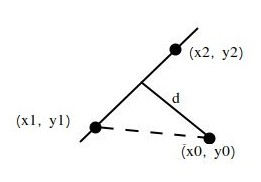
\includegraphics[width=0.5\textwidth]{dlugoscPktOdProstej}
\source{Na podstawie mathworld.wolfram.com}
\end{figure}

Wzór wyznaczający odległość punktu od prostej:

\begin{equation} \label{eq:distancePointLineal}
d = \frac{| (x_2 - x_1)(y_1 - y_0) - (x_1 - x_0)(y_2 - y_1) |}{\sqrt{(x_2 - x_1)^2 + (y_2 - y_1)^2}}
\end{equation}\newline

\begin{itemize}
\item Zmienne: x1, y1, x2, y2 oznaczają współrzędne geograficzne odpowiednio początku i końca drogi.
\item Zmienne x0, y0 oznaczają współrzędne punktu reprezentujące obiekt drogowy.
\item Zmienna d oznacza najkrótszą odleglość punktu od drogi.
\end{itemize}


\newpage
\section{Wyznaczanie współrzędnych punktu znajdującego się na drodze, odległego o n metrów od innego punktu}
\label{sec:pointCoordinatesFromAnotherPoint}

Istotnym aspektem działania algorytmu jest rozwiązanie problemu wyznaczenie współrzędnych punktu, znajdującego się na drodze, odległego o n metrów od innego punktu.  Jest to niezbędne w sytuacji, gdy np. program musi ustawić na drodze znak ograniczenia prędkości w odległosci n metrów od przejścia dla pieszych.

Do rozwiązania tego zadania, posłużyłem się własnościami trygonometrycznymi.


\begin{figure}[h]
\centering
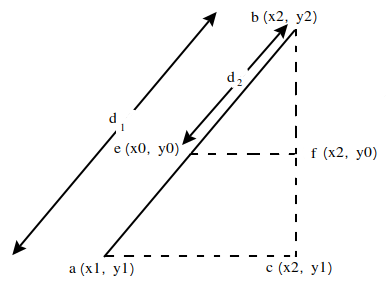
\includegraphics[width=0.5\textwidth]{distance}
\end{figure}

Odległość między dwoma punktami a i b wynosi:
\begin{equation}
d_1 = \sqrt{(x1 - x2)^2 + (y1 - y2)^2}
\end{equation}\newline

oraz sinus kąta abc:
\begin{equation}
sin_{abc} = \frac{x2 - x1}{d_1}
\end{equation}\newline

jak również sinus kąta ebf:
\begin{equation}
sin_{ebf} = \frac{x2 - x0}{d_2}
\end{equation}\newline

oraz to, że sinusy tego samego kąta są równe:
\begin{equation}
sin_{abc} = sin_{ebf} => \frac{x2 - x1}{d_1} = \frac{x2 - x0}{d_2}
\end{equation}\newline

przez proste przekształcenie, otrzymujemy wzór na współrzędną x0

\begin{equation}
x0 = x2 - \frac{d_2*(x2 - x1)}{d_1}
\end{equation}\newline

Wyznaczenie wzoru na współrzędną y0 jest podobne do wyznaczania współrzędnej x0, z tą różnicą, że zamiast sinusa, liczymy cosinusa kąta abc:

\begin{equation}
cos_{abc} = \frac{y2 - y1}{d_1}
\end{equation}\newline

oraz cosinusa kąta ebf:
\begin{equation}
cos_{ebf} = \frac{y2 - y0}{d_2}
\end{equation}\newline

a skoro cosinus tego samego kąta są równe:
\begin{equation}
cos_{abc} = cos_{ebf} => \frac{y2 - y1}{d_1} = \frac{y2 - y0}{d_2}
\end{equation}\newline

otrzymujemy równanie współrzędnej y0:
\begin{equation}
y0 = y2 - \frac{d_2*(y2 - y1)}{d_1}
\end{equation}\newline

Przez powyższe obliczenia, wyznaczone zostały wspórzędne poszukiwanego punktu:

\begin{equation} \label{eq:calculatedCoordinates}
(x2 - \frac{d_2*(x2 - x1)}{d_1}, y2 - \frac{d_2*(y2 - y1)}{d_1})
\end{equation}\newline

\newpage
\section{Wyznaczanie minimalnego obszaru pokrywającego}

W niniejszej sekcji skupię się na sposobie w jaki algorytm wyznacza minimalny obszar pokrywający (eng. minimum bounding box). Będzie on wykorzystany w późniejszych obliczeniach, mających na celu przypisanie poszczególnych dróg do danych obszarów, na których obowiązuje ograniczenie prędkości.

Rys. \ref{sec:minBoundingBoxFirst} przedstawia przykładowy wielokąt reprezentujący interesujący nas obiekt pobrany z OpenStreetMap.

\begin{figure}[h]
\caption{Przykładowy wielokąt reprezentujący obiekt na mapie}
\label{sec:minBoundingBoxFirst}
\centering
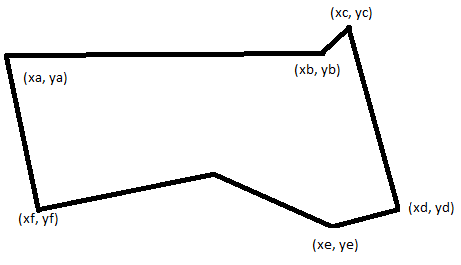
\includegraphics[width=0.8\textwidth]{minBoundingBoxFirst}
\end{figure}

W celu znalezienia minimalnego obszaru pokrywający niezbędne jest wyznaczenie czterech współrzędnych (x1, y1), (x2, y2), (x3, y3), (x4, y4) reprezentuących cztery wierzchołki prostokąta.

W celu wyznaczenia wierzchołka północno-zachodniego, należy obliczyć minimalną wartość współrzędnej x oraz maksymalną wartość współrzędnej y.

\begin{equation} \label{sec:drugiWierzcholek}
\begin{split}
x1 = min(x_a, x_b, x_c, x_d, x_e, x_f, x_g) \\
y1 = min(y_a, y_b, y_c, y_d, y_e, y_f, y_g)
\end{split}
\end{equation}\newline

Żeby wyznaczyć wierzchołek północno-wschodni, należy obliczyć maksymalną wartość współrzędnej x i y.
\begin{equation} \label{sec:trzeciWierzcholek}
\begin{split}
x2 = max(x_a, x_b, x_c, x_d, x_e, x_f, x_g)  \\
y2 = max(y_a, y_b, y_c, y_d, y_e, y_f, y_g)
\end{split}
\end{equation}\newline

Wierzchołek południowo-wschodni obliczamy jako maksymalną wartość współrzędnej x oraz minimalną wartość wsółrzędnej y.
\begin{equation} \label{sec:czwartyWierzcholek}
\begin{split}
x3 = max(x_a, x_b, x_c, x_d, x_e, x_f, x_g) \\
y3 = min(y_a, y_b, y_c, y_d, y_e, y_f, y_g)
\end{split}
\end{equation}\newline

Aby wyznaczyć południowo-zachodni wierzchołek, należy obliczyć minimalną wartość współrzędnej x i y.

\begin{equation} \label{sec:pierwszyWierzcholek}
\begin{split}
x4 = min(x_a, x_b, x_c, x_d, x_e, x_f, x_g) \\
y4 = min(y_a, y_b, y_c, y_d, y_e, y_f, y_g)
\end{split}
\end{equation}\newline

Po wyznaczeniu powyższych współrzędnych minimalny obszar pokrywający wygląda tak, jak na rysunku \ref{sec:secondtBB}


\begin{figure}[h]
\caption{Minimalny obszar pokrywający dany obiekt}
\label{sec:secondtBB}
\centering
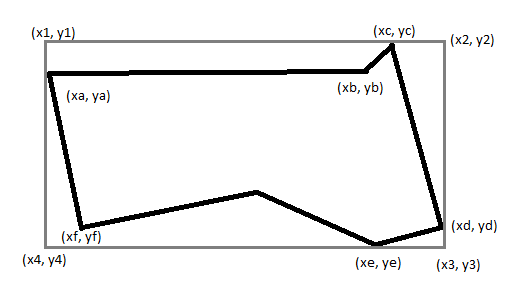
\includegraphics[width=0.9\textwidth]{minBoundingBox}
\end{figure}

\newpage
\section{Powiększanie wyznaczonego obszaru pokrywającego}

Kolejnym krokiem niezbędnym do przyporządkowania dwuwymiarowych obiektów do poszczególnych dróg jest powiększenie wyznaczonego obszaru pokrywającego. W celu wyznaczenia wierzchołków powiększonego obszaru, skorzystam z poniżej podanych równań.

\begin{equation}
\begin{split}
x1' = x1 - n \\
y1' = y1 + n \\
\end{split}
\end{equation}

\begin{equation}
\begin{split}
x2' = x2 + n \\
y2' = y2 + n \\
\end{split}
\end{equation}

\begin{equation}
\begin{split}
x3' = x3 + n \\
y3' = y3 - n \\
\end{split}
\end{equation}

\begin{equation}
\begin{split}
x4' = x4 - n \\
y4' = y4 - n \\
\end{split}
\end{equation}

Rys. \ref{sec:thirdBB} przedstawia minimalny obszar pokrywający powiększony o n metrów względem pierwotnego. Oczywiście obszar można dowolnie powiększać, w zależności od obiektu, który się w nim znajduje. Tak więc dla placów zabaw czy przedszkoli będzie znacznie większy, w porównaniu do np. przystanków autobusowych.

\begin{figure}[h]
\caption{Minimalny obszar pokrywający dany obiekt powiększony o n metrów}
\label{sec:thirdBB}
\centering
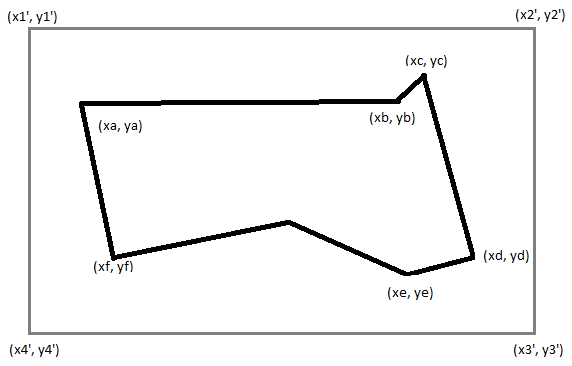
\includegraphics[width=0.7\textwidth]{BoundingBoxExtended}
\end{figure}

\newpage
\section{Łączenie powiększonych obszarów pokrywających}

W celu przyszpieszenia części algorytmu odpowiedzialnego za przypisywanie danego odcinka drogi do obszaru w którym obowiązuje ograniczenie prędkości, niezbędne jest połączenie nachodzących na siebie obszarów oraz wyznaczenie jego konturu. Można rozróżnić kilka przypadków:
\begin{itemize}
\item gdy jeden obszar całkowicie znajduje się wewnątrz drugiego
\item gdy dwa rogi obszaru mającego kształt prostokątu znajdują się wewnątrz innego obszaru
\item gdy tylko jeden róg obszaru mającego kształt prostokątu znajdje się wewnątrz innego obszaru
\end{itemize}
W niniejszych podrozdziale skupię na dokładnej metodzie wyznaczania konturu dla każdego z powyższych przypadków.

\subsection{Łączenie powiększonych obszarów pokrywających w przypadku gdy jeden obszar w całości znajduje się w drugim}

Do sytuacji w której dany obszar pokrywający w całości znajduje się wewnątrz innego obszaru dochodzi gdy np. wokół przedszkola znajduje się plac zabaw. W takiej sytuacji
można pominąć wewnętrzy obszar. Na rys \ref{fig:boundingBoxInside} został przedstawiony taki przypadek.

\begin{figure}[h]
\caption{Obszar pokrywający wewnątrz innego obszaru}
\label{fig:boundingBoxInside}
\centering
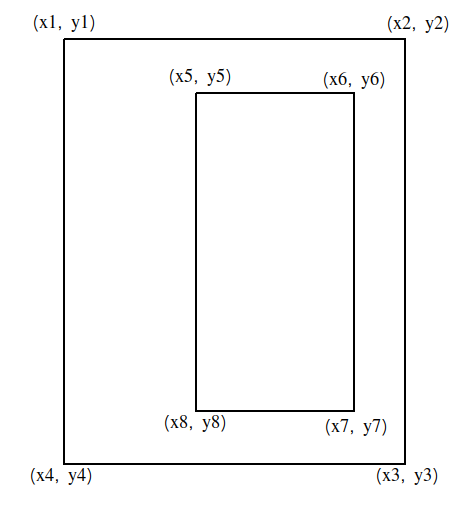
\includegraphics[width=0.6\textwidth]{boundingBoxInside}
\end{figure}

W pierwszym kroku należy znaleźć takie obszary. W tym celu algorytm iteruje po wszystkich obszarach i sprawdza, czy współrzędne spełniają wszystkie niżej przedstawione warunki.

\begin{equation}
\begin{split}
x4 <= x5 <= x2 \\
x4 <= x7 <= x2 \\
y4 <= y5 <= y2 \\
y4 <= x7 <= y2
\end{split}
\end{equation}

W następnym kroku algorytm usuwa tak znaleziony obszar. W wyniku czego na mapie pozostaje tylko obszar przestawiony na rys.\ref{fig:boundingBoxInsideRemoved}

\begin{figure}[h]
\caption{Wynik usunięcia obszaru pokrywającego wewnątrz innego obszaru}
\label{fig:boundingBoxInsideRemoved}
\centering
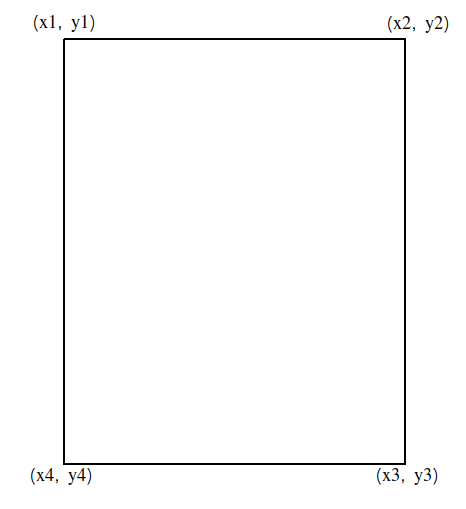
\includegraphics[width=0.6\textwidth]{boundingBoxInsideRemoved}
\end{figure}

\newpage
\subsection{Łączenie powiększonych obszarów pokrywających w przypadku gdy jeden obszar nachodzi w całości tylko jednym bokiem }

W przypadku gdy jeden obszar pokrywający w całości nachodzi tylko jednym bokiem, algorytm rozróżnia cztery możliwe sytuacje. Wszystkie one zostały przestawione na rysunku \ref{fig:OneSideBounding}.



\begin{figure}[h]
\caption{Wszystkie możliwe sytuacje w których jeden obszar nachodzi na drugi tylko jednym  bokiem}
\label{fig:OneSideBounding}
\centering
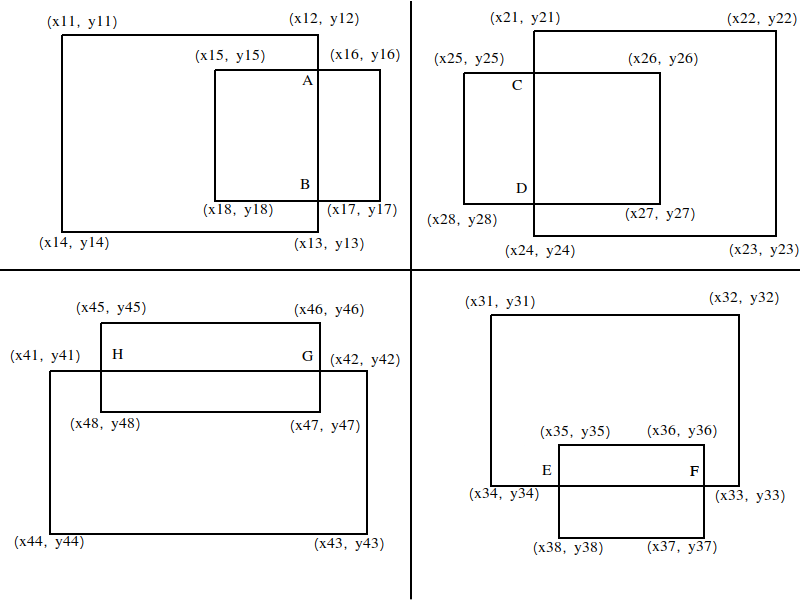
\includegraphics[width=0.8\textwidth]{OneSideBounding}
\end{figure}

W pierwszym kroku należy znaleźć takie obszary. W tym celu algorytm iteruje po wszystkich obszarach i sprawdza, czy współrzędne spełniają wszystkie niżej przedstawione warunki.

Dla pierwszej ćwiarki z rys. \ref{fig:OneSideBounding}
\begin{equation}
\begin{split}
x11 <= x15 <= x13 \\
y13 <= y15 <= y11 \\
y13 <= y18 <= y11 \\
x13 < x16 \\
\end{split}
\end{equation}

Dla drugiej ćwiarki z rys. \ref{fig:OneSideBounding}
\begin{equation}
\begin{split}
x24 <= x26 <= x22 \\
y23 <= y26 <= y21 \\
y23 <= y27 <= y21 \\
x25 < x21 \\
\end{split}
\end{equation}

Dla trzeciej ćwiarki z rys. \ref{fig:OneSideBounding}
\begin{equation}
\begin{split}
x31 <= x35 <= x33 \\
x31 <= x36 <= x33 \\
y33 <= y35 <= y11 \\
y38 < x34 \\
\end{split}
\end{equation}

Dla czwartek ćwiarki z rys. \ref{fig:OneSideBounding}
\begin{equation}
\begin{split}
x41 <= x48 <= x43 \\
x41 <= x47 <= x43 \\
y43 <= y47 <= 411 \\
y46 > x42 \\
\end{split}
\end{equation}

W następnym kroku algorytm wyznacza punkty przecięcia. Z racji tego, że nachodzące obszary są prostokątami zrotowanymi pod takim samym kątem, to do ich wyznaczenia pobiera odpowiednie współrzędne już wyznaczonych obszarów.

Dla pierwszej ćwiarki z rys. \ref{fig:OneSideBounding}

\begin{equation}
\begin{split}
A = (x12, y15) \\
B = (x12, y16)
\end{split}
\end{equation}

Dla drugiej ćwiarki z rys. \ref{fig:OneSideBounding}

\begin{equation}
\begin{split}
C = (x21, y25) \\
D = (x21, y28)
\end{split}
\end{equation}

Dla trzeciej ćwiarki z rys. \ref{fig:OneSideBounding}

\begin{equation}
\begin{split}
E = (x35, y34) \\
F = (x36, y34)
\end{split}
\end{equation}


Dla czwartej ćwiarki z rys. \ref{fig:OneSideBounding}

\begin{equation}
\begin{split}
G = (x46, y42) \\
H = (x45, y42)
\end{split}
\end{equation}

W ostatnim kroku algorytm wyznacza kontur tak przygodowanej figury, poprzez połączenie współrzędnych w odpowiedniej kolejności. Zostało to przedstawione w poniższym równaniu:

Dla pierwszej ćwiarki z rys. \ref{fig:OneSideBounding}

\begin{equation}
\begin{split}
(x11, y11) -> (x12, y12) -> (x12, y15) -> (x16, y16) ->  \\
(x17, y17) -> (x12, y16) -> (x13, y13) -> (x14, y14)
\end{split}
\end{equation}

Dla drugiej ćwiarki z rys. \ref{fig:OneSideBounding}

\begin{equation}
\begin{split}
(x21, y21) -> (x22, y22) -> (x23, y23) -> (x24, y24) ->  \\
(x21, y28) -> (x28, y28) -> (x25, y25) -> (x21, y25)
\end{split}
\end{equation}

Dla trzeciej ćwiarki z rys. \ref{fig:OneSideBounding}

\begin{equation}
\begin{split}
(x31, y31) -> (x32, 312) -> (x33, y33) -> (x36, y34) ->  \\
(x37, y37) -> (x38, y38) -> (x35, y34) -> (x34, y34)
\end{split}
\end{equation}

Dla czwartej ćwiarki z rys. \ref{fig:OneSideBounding}

\begin{equation}
\begin{split}
(x41, y41) -> (x45, y42) -> (x45, y45) -> (x46, y46) ->  \\
(x46, y42) -> (x42, y42) -> (x43, y43) -> (x44, y44)
\end{split}
\end{equation}

W wyniku powyższego algorytmu, zostały wyznaczone kontury nachodzących na siebie obszarów. Zostały przedstawione na rys. \ref{fig:OneSideBoundingRemoved}

\begin{figure}[h]
\caption{Obrys nachodzących na siebie obszarów}
\label{fig:OneSideBoundingRemoved}
\centering
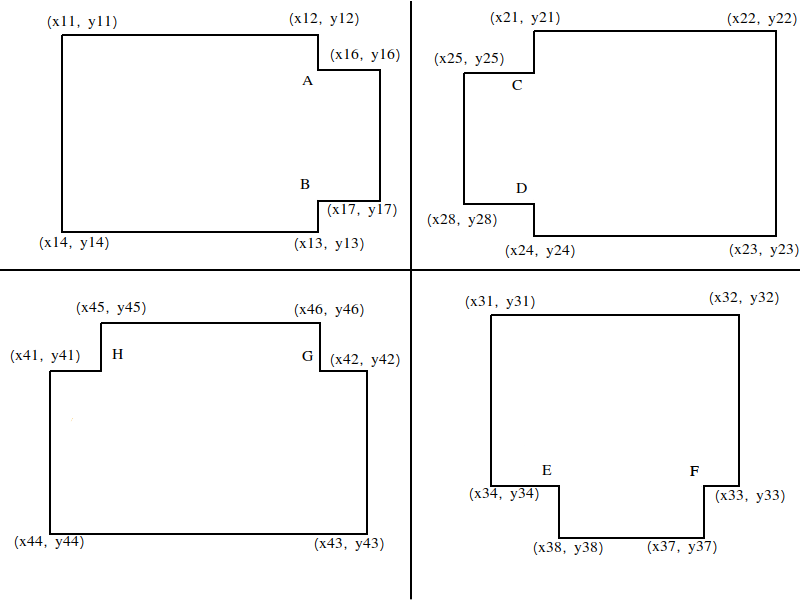
\includegraphics[width=0.75\textwidth]{OneSideBoundingRemoved}
\end{figure}

\newpage
\section{Przyporządkowanie obiektów reprezentowanych przez wielokąty, do poszczególnych dróg}
\label{sec:polygonLineDistance}

W niniejszej sekcji skupię się na rozwiązaniu problemu przyporządkowania obiektów reprezentowanych przez wielokątny do poszczególnych dróg. Wykorzystywane jest w sytuacjach, gdy trzeba określić dokładne współrzędne początku i końca strefy, na której obowiązuje ograniczonej prędkości. Obiekty na mapie, reprezentowane przez wielokąty:
\begin{itemize}
\item szkoły
\item parki
\item place zabaw
\item przystanki autobusowe i tramwajowe
\item sklepy
\item miejsca kultu
\end{itemize}




W pierwszej kolejności algorytm znajduje minimalny obszar pokrywający (eng. minimum bounding box) dany obiekt. W tym celu

\subsection{Powiększanie wyznaczonego obszaru pokrywającego}

Następnym krokiem jest powiększenie tak wyznaczonego obszaru o n metrów. Dzięki takiemu zabiegowi, możliwe będzie wyznaczenie strefy ogroniczonej prędkości.




\subsection{Łączenie powiększonych obszarów pokrywających}

W celu przyszpieszenia części algorytmu odpowiedzialnego za przypisywanie danego odcinka drogi do obszaru w którym obowiązuje ograniczenie prędkości, niezbędne jest połączenie nachodzących na siebie obszarów oraz wyznaczenie jego konturu. Można rozróżnić kilka przypadków:




\subsection{Wyznaczanie obszarów drogi znajdujących się w pobliżu interesującego nas obiektu}

Ostatnim krokiem jest wyliczenie, które drogi znajdują się o obrębie danego obszaru. Należy zaznaczyć, że Open Street Map, w przypadku łuków czy zakrętów, przedstawia je jako zbiór odcinków. Możemy tutaj wyróżnić dwa przypadki:
\begin{itemize}
\item żaden ze zbioru odcinków nie należy do danego obszaru
\item jeden lub pewna część odcinków znajduje się w obrębie danego obszaru. W takiej sytuacji należy wyznaczyć wszystkie współrzędne przecięcia, a później określić interesujące nas fragmenty drogi.
\end{itemize}


\subsubsection{Znajdowanie punktów przecięcia}

W celu znalezienia punktów przecięcia, wykorzystam fakt, że droga reprezentowana jest zbiór odcinków, oraz że interesujący nas obszar jest prostokątem - a więc posiada cztery boki.

W pierwszej kolejności algorytm będzie iterował po zbiorze odcinków. Każdy odcinek lub bok prostokąta reprezentowany jest przez dwie współrzędne:

\begin{equation}
\begin{split}
(x_a, y_a) \\
(x_b, y_b) \\
\end{split}
\end{equation}

Dzięki temu, bez problemu można określić równanie prostej przechodzącej przez te dwa punkty:

\begin{equation}
(y - y_a) (x_b-x_a) - (y_b - y_a) (x - x_a) = 0
\end{equation}

Oraz równanie w postaci kierunkowej:

\begin{equation} \label{sec:prostaKierunkowa}
y=\frac{y_a - y_b}{x_a - x_b}x + (y_a - \frac{y_a - y_b}{x_a - x_b}x_a)
\end{equation}

W celu wyznaczenia współrzędnej x punktu przecięcia wystarczy porównać oba równania:

\begin{equation}
\frac{y_c - y_d}{x_c - x_d}x + (y_c - \frac{y_c - y_d}{x_c - x_d}x_c)=\frac{y_a - y_b}{x_a - x_b}x + (y_a - \frac{y_a - y_b}{x_a - x_b}x_a)
\end{equation}

W wyniku czego otrzymujemy:

\begin{equation}
x = \frac{(y_a - \frac{y_a - y_b}{x_a - x_b}x_a) - (y_c - \frac{y_c - y_d}{x_c - x_d}x_c)}{\frac{y_c - y_d}{x_c - x_d} - \frac{y_a - y_b}{x_a - x_b}}
\end{equation}

Aby wyznaczyc współrzędną y, należy przekształcić równanie \ref{sec:prostaKierunkowa} do postaci:

\begin{equation}
x=\frac{y - (y_a - \frac{y_a - y_b}{x_a - x_b}x_a)}{\frac{y_a - y_b}{x_a - x_b}}
\end{equation}

Następnie porównać równania obu prostych:

\begin{equation}
\frac{y - (y_a - \frac{y_a - y_b}{x_a - x_b}x_a)}{\frac{y_a - y_b}{x_a - x_b}}=\frac{y - (y_c - \frac{y_c - y_d}{x_c - x_d}x_c)}{\frac{y_c - y_d}{x_c - x_d}}
\end{equation}

W wyniku czego otrzymujemy wzór na współrzędną y przecinającą obie proste:
\begin{equation}
y = \frac{(y_a - \frac{y_a - y_b}{x_a - x_b}x_a)(\frac{y_c - y_d}{x_c - x_d}) - (\frac{y_a - y_b}{x_a - x_b})(y_c - \frac{y_c - y_d}{x_c - x_d}x_c)}
{(\frac{y_c - y_d}{x_c - x_d})(\frac{y_a - y_b}{x_a - x_b})}
\end{equation}

\subsubsection{Sprawdzanie, czy punkt przecięcia należy do odcinka}

W celu sprawdzenia, czy punkt przecięcia należy do odcinka, posłużę się własnością, że suma długości mierzonej od początku odcinka do danego punktu oraz od danego punktu, do końca odcinka jest równa całkowitej długości odcinka.

\begin{equation} \label{eq:pointInSegment}
|AC| + |CB| = |AB|
\end{equation}

W celu lepszego zobrazowania, posłuże się rysunkiem \ref{sec:pointSegment}

\newpage
\begin{figure}[h]
\caption{Punkt wewnątrz odcinka}
\label{sec:pointSegment}
\centering
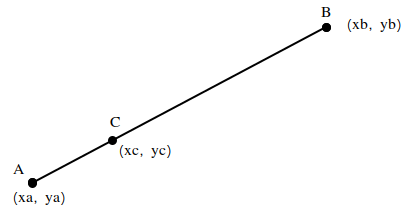
\includegraphics[width=0.6\textwidth]{pointInSegment}
\end{figure}

Odległość między dwoma punktami a i b wynosi:
\begin{equation}
d = \sqrt{(x1 - x2)^2 + (y1 - y2)^2}
\end{equation}\newline

Długość odcinka AC wynosi:

\begin{equation} \label{eq:distanceBetweenTwoPointAC}
d_{AC} = \sqrt{(xa - xc)^2 + (ya - yc)^2}
\end{equation}\newline

Długość odcinka CB wynosi:
\begin{equation} \label{eq:distanceBetweenTwoPointCB}
d_{CB} = \sqrt{(xc - xb)^2 + (yc - yb)^2}
\end{equation}\newline

Oraz długość odcinka AB wynosi:
\begin{equation}
d_{AB} = \sqrt{(xa - xb)^2 + (ya - yb)^2}
\end{equation}\newline

Zgodnie z równaniem \ref{eq:pointInSegment}, aby punkt nalezał do odcinka, musi spełniać warunek:

\begin{equation}
\sqrt{(xa - xb)^2 + (ya - yb)^2} = \sqrt{(xa - xb)^2 + (ya - yb)^2} + \sqrt{(xc - xb)^2 + (yc - yb)^2}
\end{equation}\newline

\subsubsection{Wyznaczenie obszarów drogi znajdujących się w pobliżu danego obiektu}



\newpage
\begin{figure}[h]
\caption{Droga przebiegająca przez wybrany obszar}
\label{sec:fourthBB}
\centering
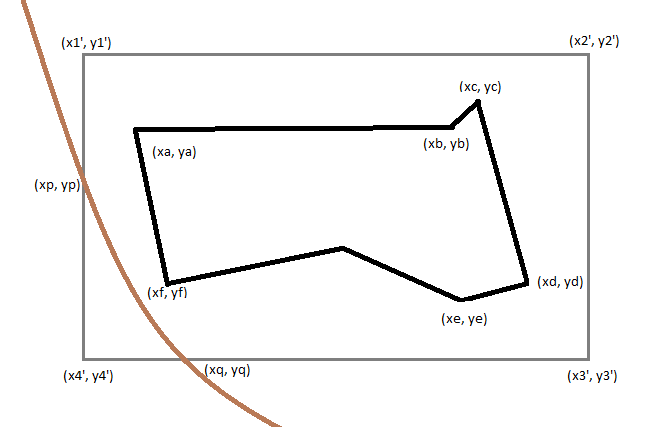
\includegraphics[width=0.8\textwidth]{minBoundingBoxWay}
\end{figure}

\newpage
\section{Przejścia dla pieszych}
\label{sec:pedestrialCrossing}
\subsection{Przyporządkowywanie przejść dla pieszych do poszczególnych dróg}

Bardzo ważnym czynnikiem doboru prędkości jest obecność przejść dla pieszych. Te z sygnalizacją świetlną nie stanowią problemu, ponieważ ruch pieszych poruszających się na nich jest ograniczony tylko do sytuacji, gdy sygnalizacja świeci się na zielono. W przypadku przejść bez sygnalizacji, sprawa się komplikuje, ponieważ kierowca jest zobowiązany do zachowania szczególnej ostrożności i zmiejszenia prędkości od 30 km/h.

Do przyporządkowania przejść dla pieszych, do poszczególnych dróg, posłużyłem się wzorem \ref{eq:distancePointLineal} na odległość punktu od prostej, przedstawionym w sekcji \ref{sec:ObiektyPunktDrogi}.


Rezultatem wdrożenia powyższego wzoru do programu, są:
\begin{itemize}
\item na niebiesko zaznaczone drogi, na których znajdują się przejścia dla pieszych
\item znakiem ''D-6'' zostały oznaczone przejścia dla pieszych
\end{itemize}
Wynik został przedstawiony na Rys. \ref{sec:PrzejscieDrogi}:

\begin{figure}[h]
\caption{Drogi na których znajdują się przejścia dla pieszych.}
\label{sec:PrzejscieDrogi}
\centering
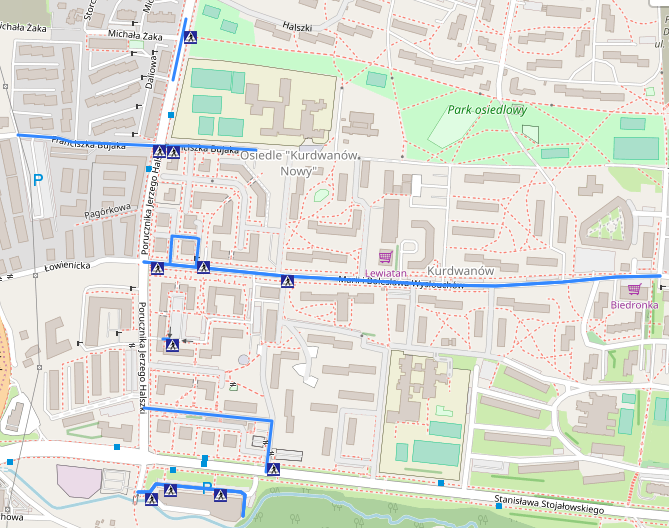
\includegraphics[width=0.9\textwidth]{PrzejscieDrogi}
\end{figure}

Dzięki tak zobrazowanej sytuacji, można ocenić skuteczność algorytmu przyporządkowującego przejścia dla pieszych do określonych dróg.

\subsection{Wyznaczanie prędkości i umieszczanie jej w odpowiednim miejscu na mapie}

Bezpieczna prędkość w pobliżu nieoznakowanych przejść dla pieszych wynosi ok. 30 km/h. Zapewnia ona zarówno wystarczajacy czas reakcji, odpowiednio krótką drogę hamowania oraz zmiejsza ryzyko wystąpień potrąceń pieszych.

Algorytm umieszcza znaki ograniczenia prędkości:
\begin{itemize}
\item w odległości 50 m od przejścia, gdy maksymalna prędkość na drodze wynosi 60 km/h
\item w odległości 150 m od przejścia, gdy maksymalna prędkość przekracza 60 km/h
\item w przypadku, gdy przejście dla pieszych znajduje się w odległości mniejszej niż 50m lub 150m (w zależności od maksymalnej prędkości), znak zostanie umieszczony na początku drogi
\item w przypadku drogi jednokierunkowej, tylko przed przejściem
\item w przypadku drogi dwukierunkowej, zarówno przed, jak i za przejściem
\item bezpośrednio za przejściem zostanie ustawiony znak przywracającą poprzednie ograniczenie prędkości, za wyjątkiem sytuacji, gdy droga za przejściem dla pieszych jest krótsza niż 100m. W takim wypadku, nie ma sensu zmieniać prędkości.
\end{itemize}

\begin{figure}[h]
\caption{Ograniczenia prędkości przy przejściach dla pieszych.}
\label{sec:przejsciePredkosci}
\centering
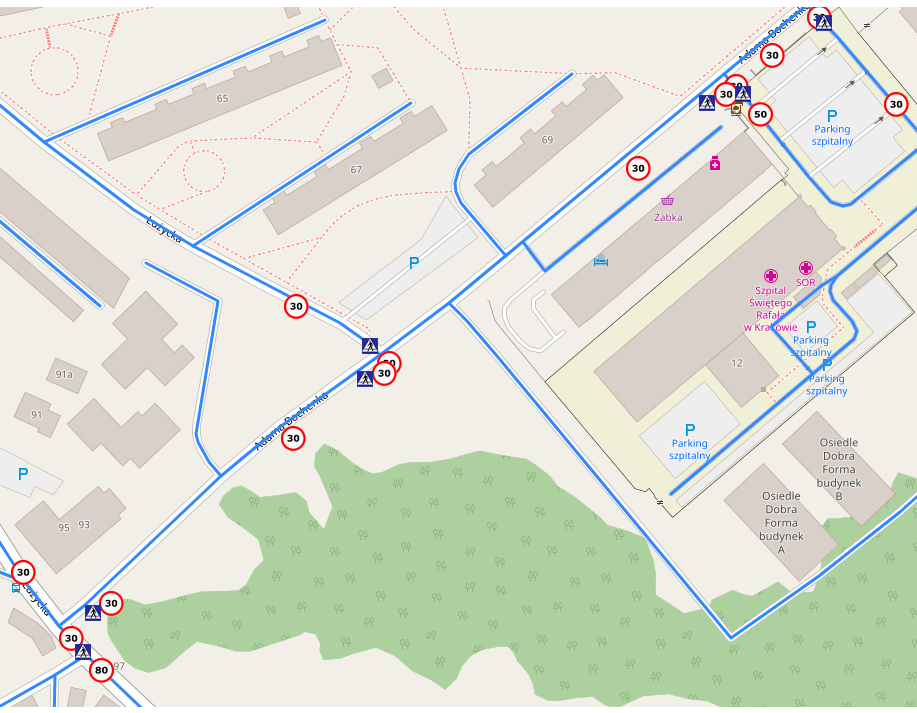
\includegraphics[width=0.9\textwidth]{pedestrian_speed}
\end{figure}

\newpage
\section{Typ nawierzchni}
\label{sec:surfaceType}

W celu zadbania o bezpieczeństwo osób, ale również o dobrą kondycję techniczną pojazdów poruszających się po drogach, niezbędne jest uwzględnienie typu nawierzchni. Nie można dopuścić do sytuacji, gdy na nawierzchni składającej się głównie że żwiru, znajdowało się znak ograniczenia prędkości o wysokiej wartości. Wtedy ulec awarii może zarówno zawieszenie, jak również pojazdy jadące przed nimi pojazdami. Aby zapoabiec tego typu problemom, podzieliłem typ nawierzchni na kilka rodzajów:

\begin{itemize}
\item kostka brukowa
\item żwir
\item drobny żwir
\item nieutwardzana
\item błotnista
\item płyty  betowowe
\item droga gruntowa
\item piasek
\item asfalt
\end{itemize}

Najbardziej problematyczna dla kierowów droga to taka, która pokryta jest żwirem, drobnym żwirem, składająca się z piasku lub jest błotnista. W takich przypadkach ograniczyłem prędkość do 10 km/h. Niewiele lepsza nawierzchnia to taka, która wyłożona jest zarówno kostką brukową oraz płytami betonowymi. Dla nich, odpowiednia prędkość wynosi 20 km/h. W przypadku drogi nieutwardzanej oraz gruntowej, ograniczenie prędkości wynosi 30 km/h. Dla asfaltu, ze względu na jego strukturę, ograniczenie prędkości praktycznie nie występuje.

Na Rys. \ref{sec:surfaceTypePhoto} zostały umieszczone ograniczenia prędkości dla dróg, których nawierzchnia pokryta jest materiałem innym niż asfalt. Dla celów demonstracyjnych, został on specjalnie pominięty, ponieważ więszkość dróg jest nim pokryta, przez co Rys. \ref{sec:surfaceTypePhoto} stałby się mało czytelny. Oczywiście ogólny algorytm uwzględnia asfalt.

\newpage
\begin{figure}[h]
\caption{Ograniczenia prędkości ze względu na rodzaj nawierzchni.}
\label{sec:surfaceTypePhoto}
\centering
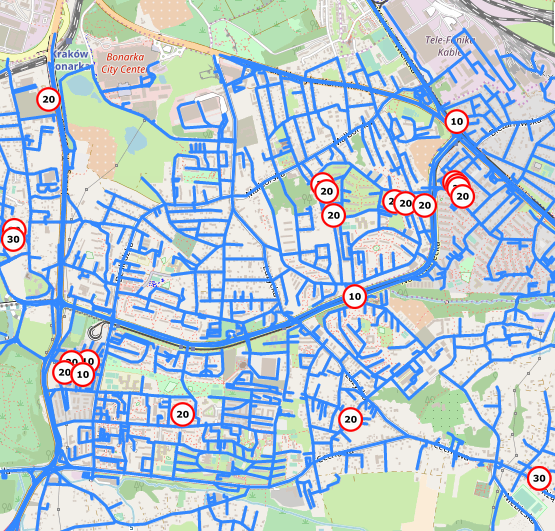
\includegraphics[width=0.9\textwidth]{surfaceType}
\end{figure}

\newpage
\section{Przejazdy kolejowe}
\subsection{Przyporządkowywanie przejazdów kolejowych do poszczególnych dróg}

Istotnych parametrem algorytmu wyznaczającego dopuszczalne prędkości jest obecność przejazdów kolejowych. Jak wiadomo, pociąg nie zatrzyma się w miejscu. Jego droga chamowania w głównej mierze zależy od masy oraz prędkości z jaką się porusza. Dla przykładu, pociąg towarowy o masie ok. 1800 ton, jadący z prędkością ok. 50 km/h, zatrzyma sie po około 500m. Dlatego ważne jest określenie prędkości, z jaką samochód moze się przemieszczać przed takim przejazdem.

Do przyporządkowania przejazdów kolejowych do poszczególnych dróg, wykorzystałem wzór \ref{eq:distancePointLineal} znajdujący się w rozdziale \ref{sec:pedestrialCrossing}


\begin{figure}[h]
\caption{Drogi na których znajdują się przejazdy kolejowe.}
\label{sec:PrzejazdyKolejowe}
\centering
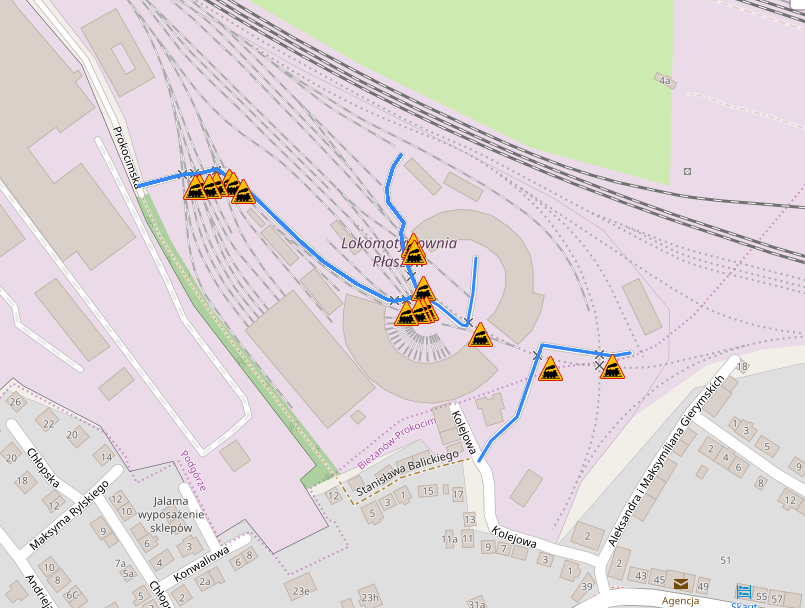
\includegraphics[width=1.0\textwidth]{railCrossing}
\end{figure}

Rys. \ref{sec:PrzejazdyKolejowe} obrazuje wynik przypisania przejazdów kolejowych do poszczególnych dróg:
\begin{itemize}
\item kolorem niebieskim drogi, na ktorych znajdują przejazdy kolejowe
\item znakiem ''A-10'' zostały oznaczone przejazdy kolejowe, pobrane z OpenStreetMap
\end{itemize}

\newpage
\subsection{Wyznaczanie prędkości i umieszczanie jej w odpowiednim miejscu na mapie}

Podobnie jak miało to miejsce w rozdziale \ref{sec:pedestrialCrossing}, umiejscowienie znaków przed przejazdem będzie zależało od kilku czynników:
\begin{itemize}
\item na  drodze z ograniczeniem prędkości do 60 km/h, znak zostanie umieszczony 50m przed przejazdem kolejowym
\item w przypadku prędkości powyżej 60 km/h, znak zostanie umieszczony w odległości 150m przed przejazdem kolejowym
\item w przypadku drogi jednokierunkowej, tylko przed przejazdem kolejowym
\item w przypadku drogi dwukierunkowej, zarówno przed, jak i za przejazdem
\item bezpośrednio za przejazdem zostanie ustawiony znak przywracającą poprzednie ograniczenie prędkości, za wyjątkiem sytuacji, gdy droga za przejazdem kolejowym jest krótsza niż 100m. W takim wypadku, nie ma sensu zmieniać prędkości.
\end{itemize}

Rys. \ref{sec:PrzejazdyKolejowe1} obrazuje przejazd kolejowy znajdujący się na dwukierunkowej drodze, na której obowiązuje ograniczenie prędkości do 80 km/h. Dlatego znaki 30 km/h zostały umieszczone 150m przed przejazdem, a zaraz po nim znaki przywracające poprzednią prędkość 80 km/h. Znaki są po obu stronach, gdyż jest do droga dwukierunkowa

\begin{figure}[h]
\caption{Umiejscowienie znaków przed i za przejazdem kolejowym.}
\label{sec:PrzejazdyKolejowe1}
\centering
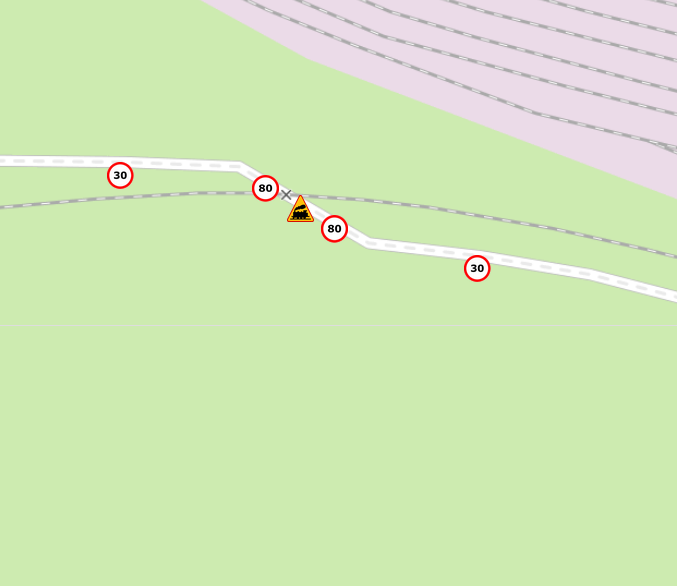
\includegraphics[width=0.7\textwidth]{streetBeforeRail}
\end{figure}


\newpage
\section{Sygnalizacja świetlna}
\subsection{Przyporządkowywanie sygnalizacji świetlnej do poszczególnych dróg}

Aby kierowca bez problemu mógł zdążyć zareagować na zmieniające się swiatło sygnalizacji świetlnej, niezbędne jest zredukowanie prędkości do odpowiedniej wartości. Ze względu na fakt iż sygnalizacja widoczna jest z relatywnie dużej odległości, prędkość przed nią zostanie ograniczona do ok. 50 km/h.


\begin{figure}[h]
\caption{Drogi na których znajduje się sygnalizacja świetlna.}
\label{sec:PrzejazdyKolejowe2}
\centering
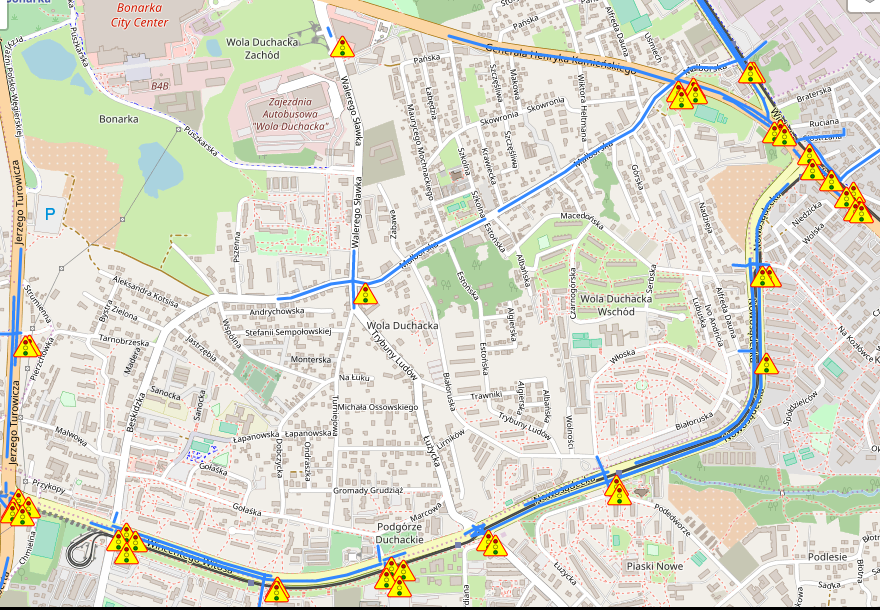
\includegraphics[width=1.1\textwidth]{traffic_sight}
\end{figure}

Rys. \ref{sec:PrzejazdyKolejowe2} ukazuje sposób działania algorytmu przypisującego do drogi sygnalizację świetlną. Zaznaczono na nim:
\begin{itemize}
\item kolorem niebieskim drogi, na ktorych znajduje się sygnalizacja świetlna
\item znakiem ''A-29'' zostały oznaczone sygnalizacje świetlne, pobrane z OpenStreetMap
\end{itemize}

\newpage
\subsection{Wyznaczanie prędkości i umieszczanie jej w odpowiednim miejscu na mapie}

Algorytm umieszcza znaki ograniczenia prędkości w następujący spasób:
\begin{itemize}
\item 50m przed sygnalizacją na drodze z ograniczeniem prędkości do 60 km/h
\item 150m przed sygnalizacją na drodze z ograniczeniem prędkości powyżej 60 km/h
\item w przypadku drogi dwukierunkowej, zarówno przed, jak i za przejazdem
\end{itemize}


Rys. \ref{sec:znakiSwiatla} obrazuje fragment skrzyżowania na której znajduje się sygnalizacja świetlna. Ograniczenie prędkości na drogach wynosi od 70 do 80 km/h, dlatego algorytm umieścił znak ograniczenia prędkości do 50 km/h, 150m przed sygnalizacją oraz znak przywracający poprzednią prędkość zaraz za sygnalizacją.

\begin{figure}[h]
\caption{Ograniczenie predkości przed i za światłami drogowymi}
\label{sec:znakiSwiatla}
\centering
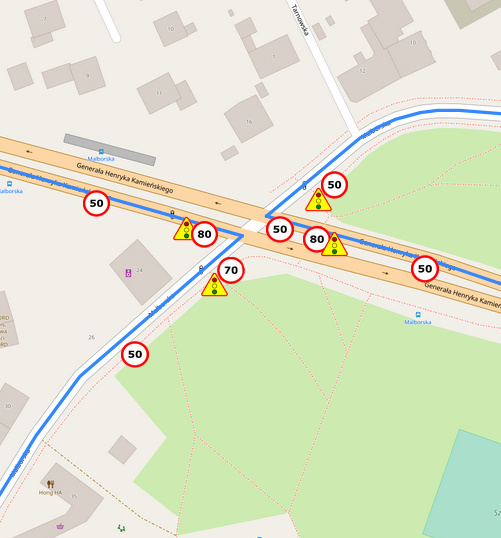
\includegraphics[width=0.8\textwidth]{speedBeforeSignals}
\end{figure}

\newpage
\section{Przystanki autobusowe i tramwajowe}


\newpage
\section{Szkoły i miesca zabaw}


\newpage
\section{Sklepy i miejsca kultów religijnych}


\newpage
\section{Liczba pasów ruchu}


\newpage
\section{Rodzaj drogi}


\newpage
\section{Płynna zmiana prędkości pojazdów}


\newpage
\section{Historia wypadków}


\newpage
\section{Zakręty}


\section{Umiejscowienie znaków na drodze}
\label{sec:speedLimitLocalization}
Znaki drogowe ograniczenia prędkości są ustawione według następujących kryteriów:
\begin{itemize}
\item na początku każdej drogi
\item przed nieoznakowanymi przejściami dla pieszych
\item przed wjazdem do obszaru, w pobliżu którego znajdują się szkoły, place zabaw, duże sklepy handlowe i miejsca kultów religijnych
\item przed zakrętami
\item między znakami ograniczenia prędkości, dla których występują duże różnice prędkości
\end{itemize}

